% This file was created with tikzplotlib v0.10.1.post5.
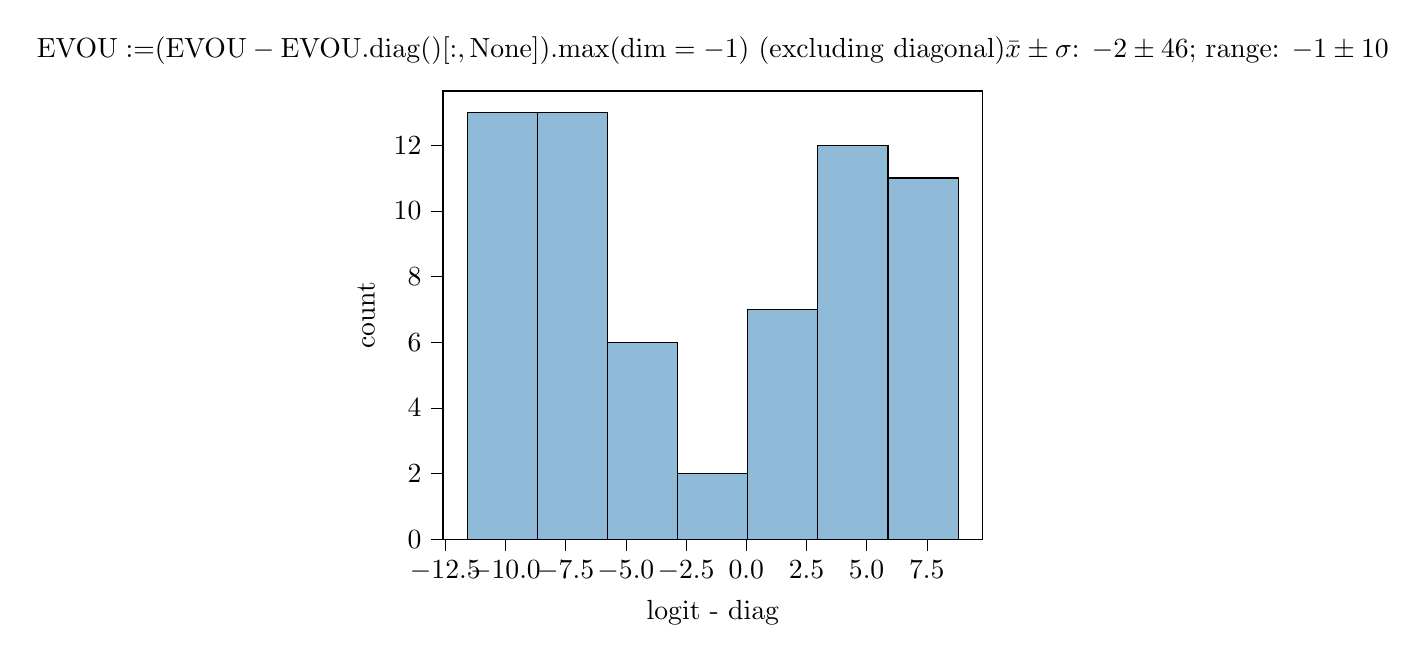
\begin{tikzpicture}

\definecolor{darkgray176}{RGB}{176,176,176}
\definecolor{steelblue31119180}{RGB}{31,119,180}

\begin{axis}[
tick align=outside,
tick pos=left,
title={\(\displaystyle \mathrm{EVOU} := \WE \WV \WO\WU \)\\
\(\displaystyle (\mathrm{EVOU} - \mathrm{EVOU}\mathrm{.diag}()[:,\mathrm{None}])\mathrm{.max}(\mathrm{dim}=-1)\) (excluding diagonal)\\
\(\displaystyle \bar{x}\pm\sigma\): \(\displaystyle -2 \pm 46\); range: \(\displaystyle -1 \pm 10\)},
x grid style={darkgray176},
xlabel={logit - diag},
xmin=-12.5941515922546, xmax=9.81734762191772,
xtick style={color=black},
xtick={-15,-12.5,-10,-7.5,-5,-2.5,0,2.5,5,7.5,10},
xticklabels={
  \(\displaystyle {\ensuremath{-}15.0}\),
  \(\displaystyle {\ensuremath{-}12.5}\),
  \(\displaystyle {\ensuremath{-}10.0}\),
  \(\displaystyle {\ensuremath{-}7.5}\),
  \(\displaystyle {\ensuremath{-}5.0}\),
  \(\displaystyle {\ensuremath{-}2.5}\),
  \(\displaystyle {0.0}\),
  \(\displaystyle {2.5}\),
  \(\displaystyle {5.0}\),
  \(\displaystyle {7.5}\),
  \(\displaystyle {10.0}\)
},
y grid style={darkgray176},
ylabel={count},
ymin=0, ymax=13.65,
ytick style={color=black},
ytick={0,2,4,6,8,10,12,14},
yticklabels={
  \(\displaystyle {0}\),
  \(\displaystyle {2}\),
  \(\displaystyle {4}\),
  \(\displaystyle {6}\),
  \(\displaystyle {8}\),
  \(\displaystyle {10}\),
  \(\displaystyle {12}\),
  \(\displaystyle {14}\)
}
]
\draw[draw=black,fill=steelblue31119180,fill opacity=0.5] (axis cs:-11.5754470825195,0) rectangle (axis cs:-8.66486276899065,13);
\draw[draw=black,fill=steelblue31119180,fill opacity=0.5] (axis cs:-8.66486276899065,0) rectangle (axis cs:-5.75427845546177,13);
\draw[draw=black,fill=steelblue31119180,fill opacity=0.5] (axis cs:-5.75427845546177,0) rectangle (axis cs:-2.8436941419329,6);
\draw[draw=black,fill=steelblue31119180,fill opacity=0.5] (axis cs:-2.8436941419329,0) rectangle (axis cs:0.0668901715959827,2);
\draw[draw=black,fill=steelblue31119180,fill opacity=0.5] (axis cs:0.0668901715959827,0) rectangle (axis cs:2.97747448512486,7);
\draw[draw=black,fill=steelblue31119180,fill opacity=0.5] (axis cs:2.97747448512486,0) rectangle (axis cs:5.88805879865374,12);
\draw[draw=black,fill=steelblue31119180,fill opacity=0.5] (axis cs:5.88805879865374,0) rectangle (axis cs:8.79864311218262,11);
\end{axis}

\end{tikzpicture}
